\begingroup
\begin{figure*}[ht]
\centering
\setlength{\fboxrule}{1pt}
\setlength{\fboxsep}{0pt}
\hspace{-0.1in}
	\begin{subfigure}[b]{0.3\textwidth}
		{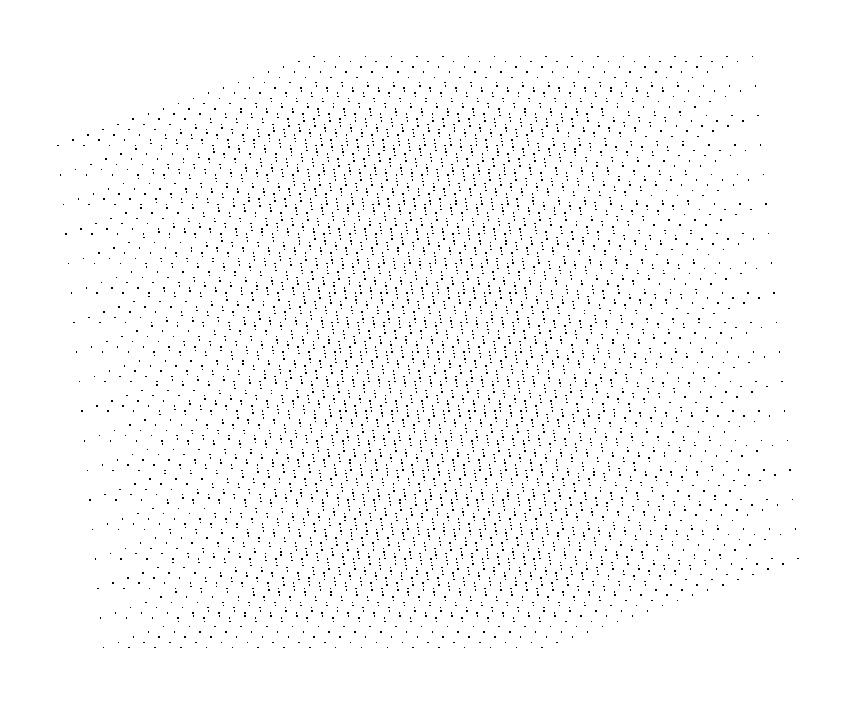
\includegraphics[width=\textwidth]{p5832.pdf}}
		\subcaption[]{5,832 particles (6000 fps)}
		\label{fig:p5832}
	\end{subfigure}
\hspace{-0.1in}
	\begin{subfigure}[b]{0.3\textwidth}
		{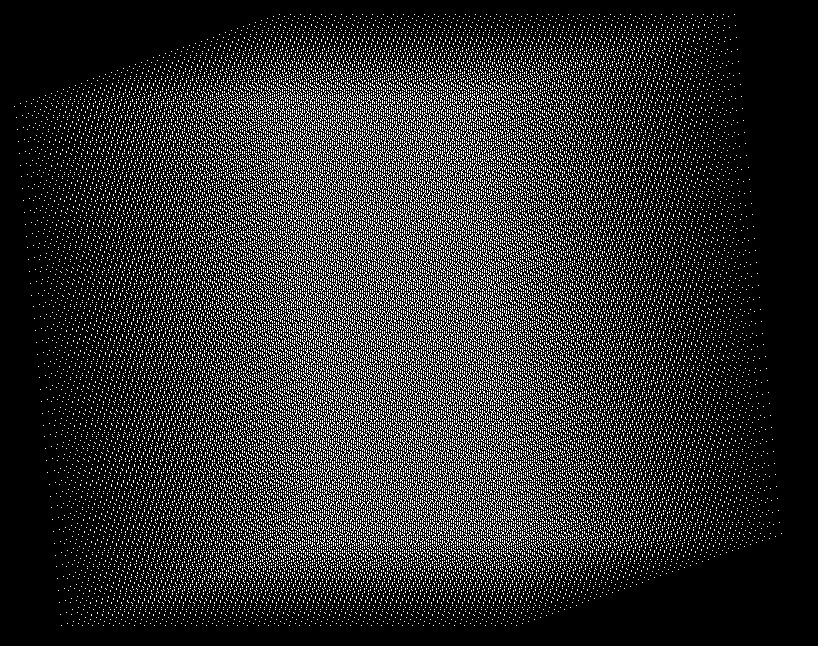
\includegraphics[width=\textwidth]{p91125.pdf}}
		\subcaption[]{91,125 particles (1700 fps)}
		\label{fig:p91125}
	\end{subfigure}
\hspace{-0.1in}
	\begin{subfigure}[b]{0.3\textwidth}
		{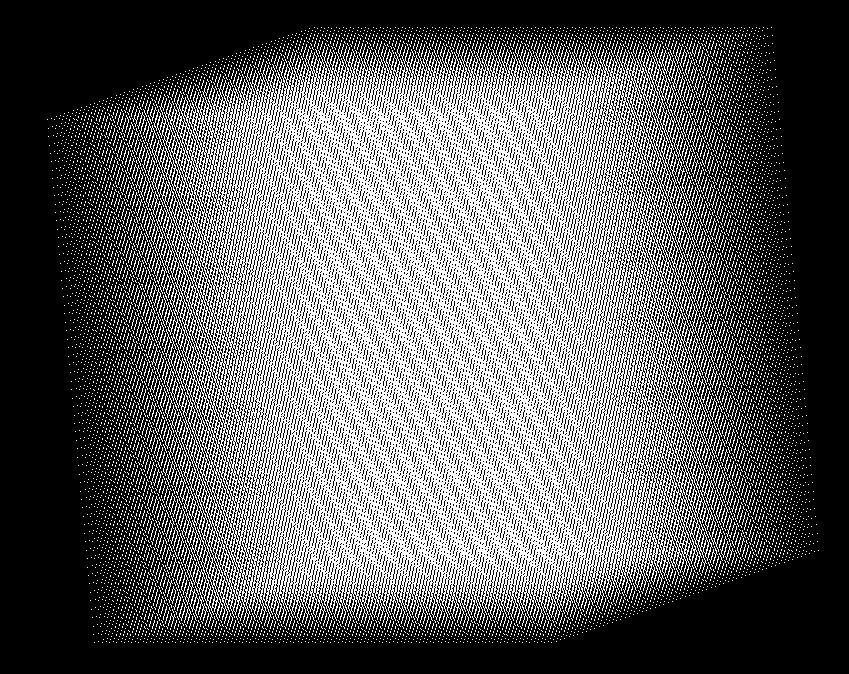
\includegraphics[width=\textwidth]{p250047.pdf}}
		\subcaption[]{250,047 particles (860 fps)}
		\label{fig:p250047}
	\end{subfigure}
\hspace{-0.1in}
	\begin{subfigure}[b]{0.3\textwidth}
		{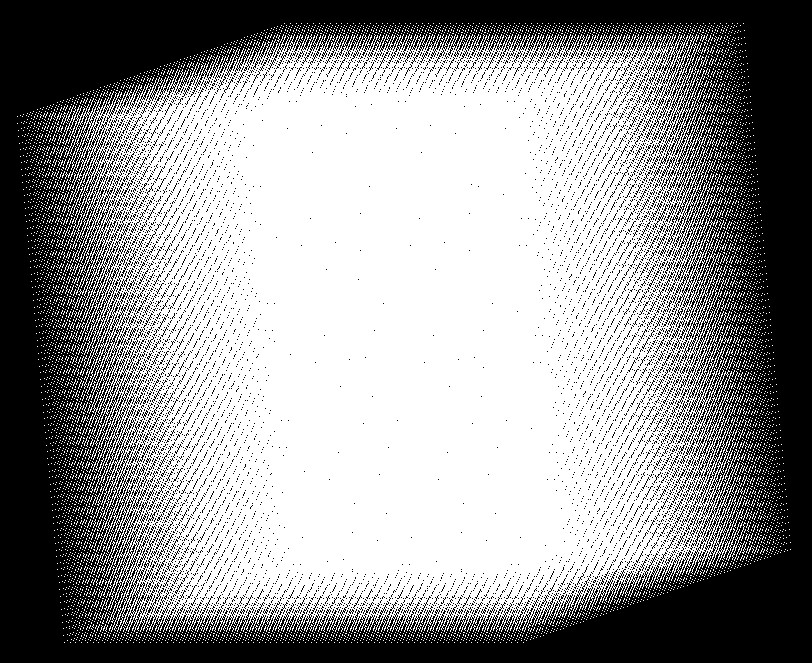
\includegraphics[width=\textwidth]{p531441.pdf}}
		\subcaption[]{531,441 particles (299 fps)}
		\label{fig:p531441}
	\end{subfigure}
\hspace{-0.1in}
	\begin{subfigure}[b]{0.3\textwidth}
		{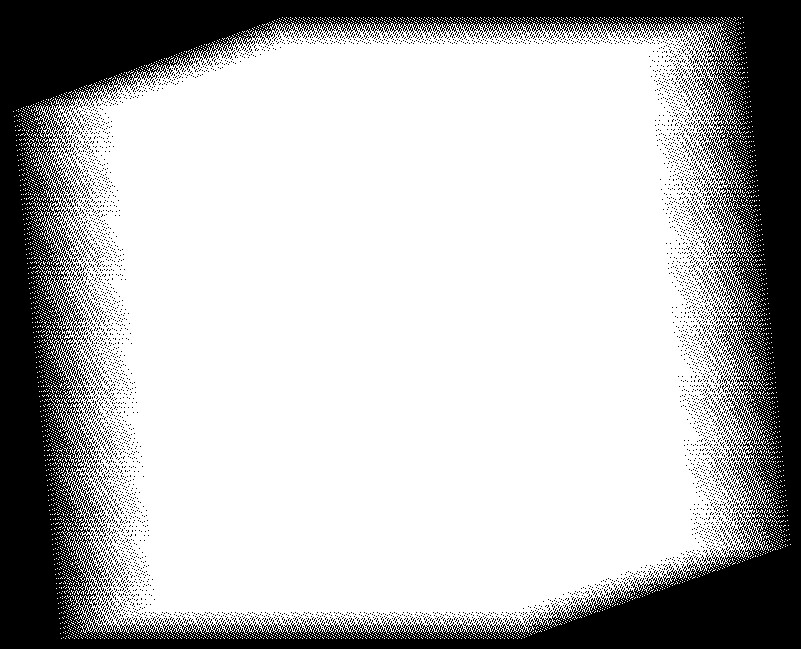
\includegraphics[width=\textwidth]{p1259712.pdf}}
		\subcaption[]{1,259,712 particles (130 fps)}
		\label{fig:p1259712}
	\end{subfigure}
\hspace{-0.1in}
	\begin{subfigure}[b]{0.3\textwidth}
		{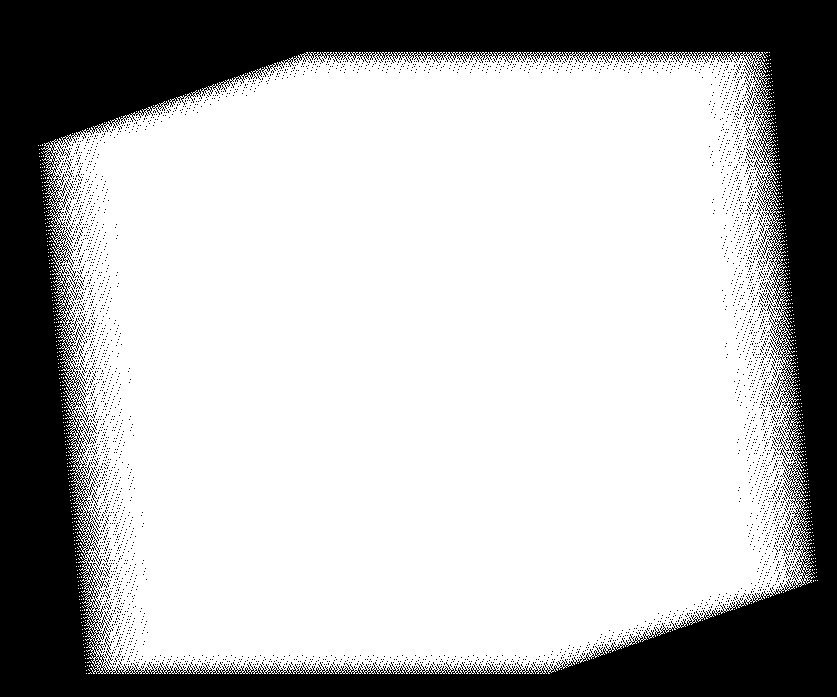
\includegraphics[width=\textwidth]{p2985984.pdf}}
		\subcaption[]{2,985,948 particles (48 fps)}
		\label{fig:p2985984}
	\end{subfigure}
\caption[TITLE:Cell Spans]{Frame captures illustrating particle
distributions at increasing densities with estimted frame rate. 
The examples shown were generated by maintaining a fixed (10x10x10) cell array
while increasing the number of particles occupying each cell. Similar
particle counts can also be achieved by increasing the size of the cell
array while maintaining a lower particle occupancy per cell. The latter
configuration is generally preferred because it reduces local cell
occupancy and therefore decreases the number of candidate interactions
evaluated during narrow-phase collision detection. This behavior aligns
well with the gPCD architecture, which benefits from distributing
particles across a larger number of cells rather than increasing the
number of particles contained within each cell.}

\label{fig:DensityGraphs}
\end{figure*}
\endgroup